\subsection{Generalized Matched Filter Detector}
\label{sec:detector}

Model-based magnetic anomaly detection showed a robustness for dipole detection \cite{https://doi.org/10.1049/rsn2.70091}. Those detection problems are usually formulated as the detection of known signals with unknown amplitudes embedded in noise, assuming an additive white Gaussian noise (AWGN). The optimal solution to this kind of problem becomes a Generalized matched filter (GMF) combined with a Generalized likelihood ratio test (GLRT) \cite{Kay1998Detection}.

The orthogonality of the chosen basis functions ensures that the signal components are uncorrelated. This property significantly simplifies the GMF structure by reducing it to two independent matched filters, one for each basis function. Under these conditions, and regarding equation~\eqref{eq:anomaly_final} the GLRT can be formulated with the following hypotheses:
\begin{align*}
\mathcal{H}_0 &: X(\tau) = w(\tau)\\
\mathcal{H}_1 &: X(\tau) = A_1 \Phi_1(\tau) + A_2 \Phi_2(\tau) + w(\tau)
\end{align*}
where \(A_1\) and \(A_2\) are the unknown signal amplitudes, \(\Phi_1(\tau)\) and \(\Phi_2(\tau)\) are the orthonormal basis functions and the signal templates for the matched filters, and \(w(\tau) \sim \mathcal{N}(0, \sigma^2)\) represents the noise.


We note that in practice, we de-normalize the basis functions (so they become a function of time $t$), reducing the calculation needed to normalize the input signal $X(t)$. The corresponding detection procedure and statistical characterization are illustrated in Figure~\ref{fig:filter_diagram}.
\begin{figure}
    \centering
    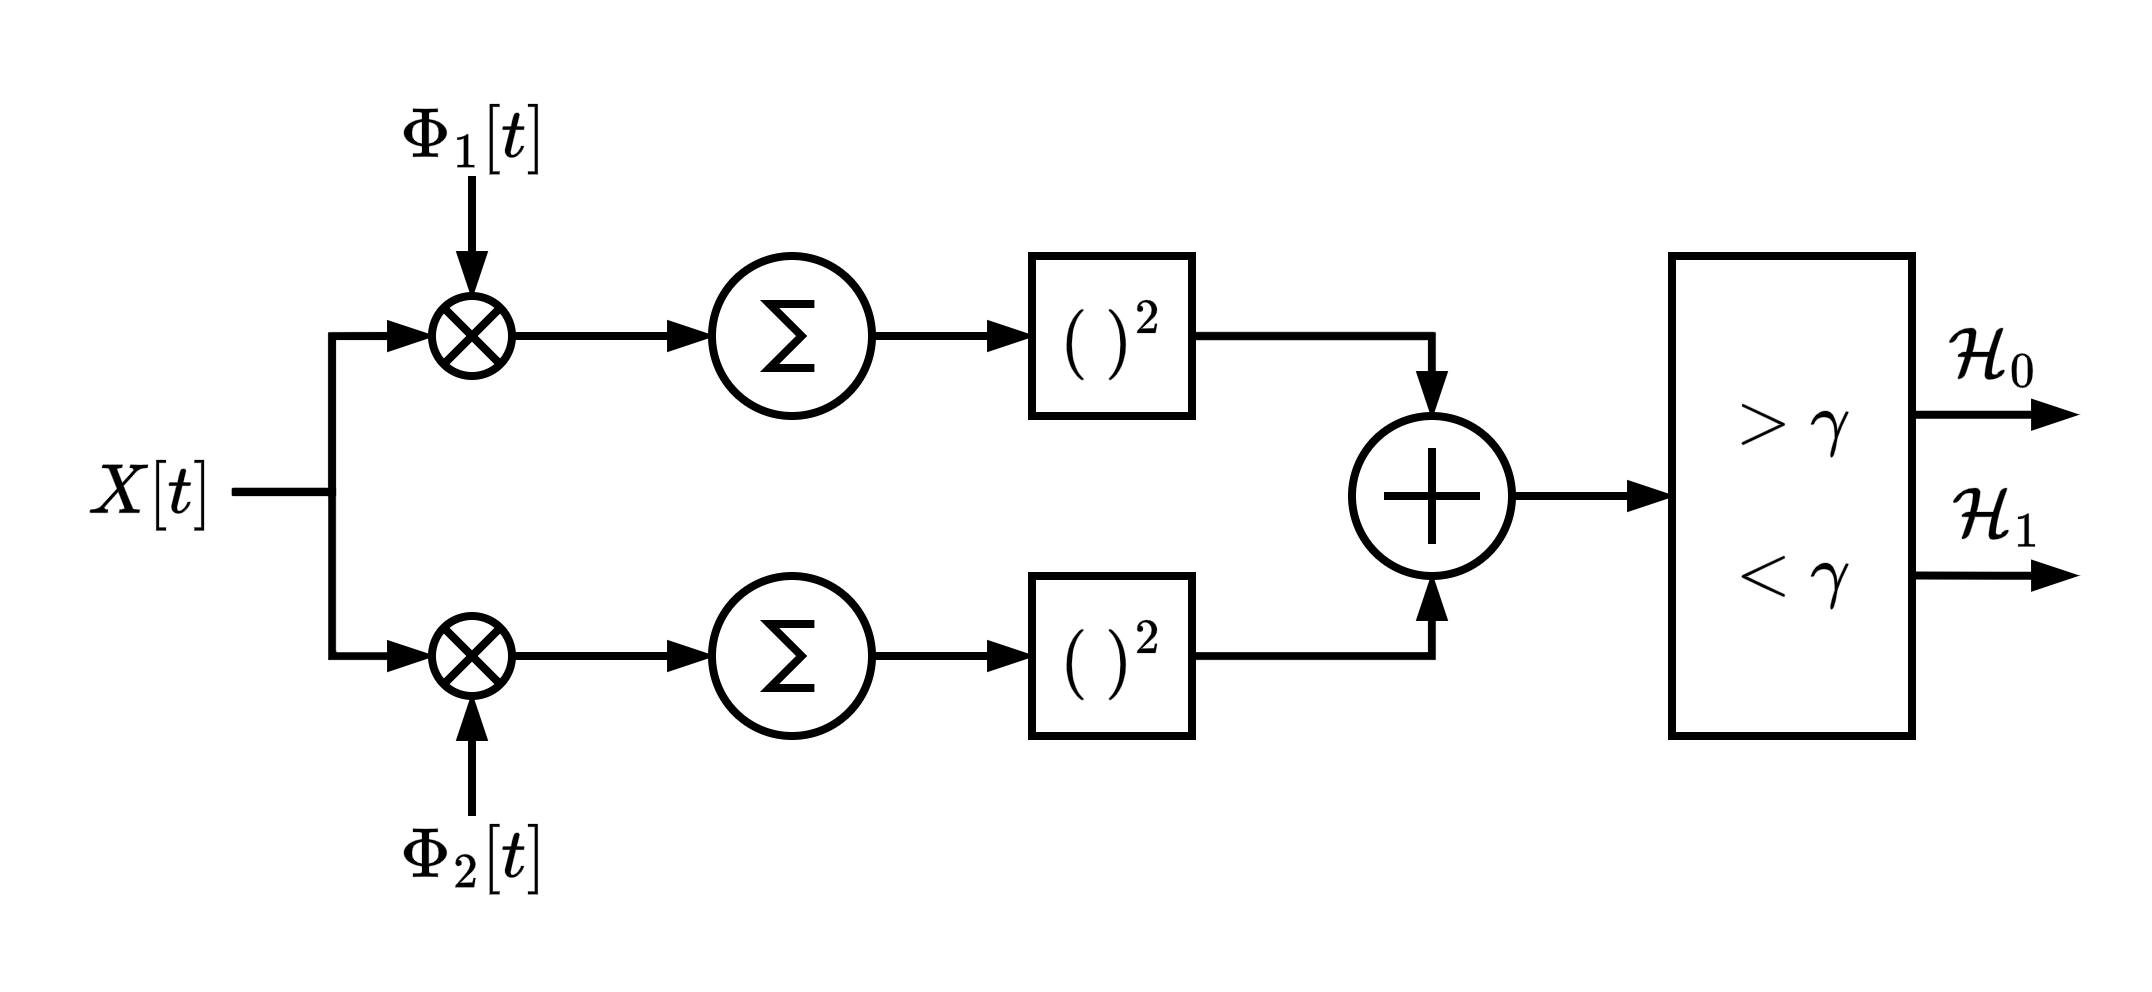
\includegraphics[width=1\linewidth]{methodology//figures/filter_diagram.png}
    \caption{diagram of the matched filter and hypothesis test used for magnetic anomaly detection}
    \label{fig:filter_diagram}
\end{figure}

\highlight{In the remainder of this work, experiments were conducted to determine under which conditions the proposed cable OBF method outperforms the established MOBF approach for the task of cable detection.}